\begin{figure}[htp]
\centering
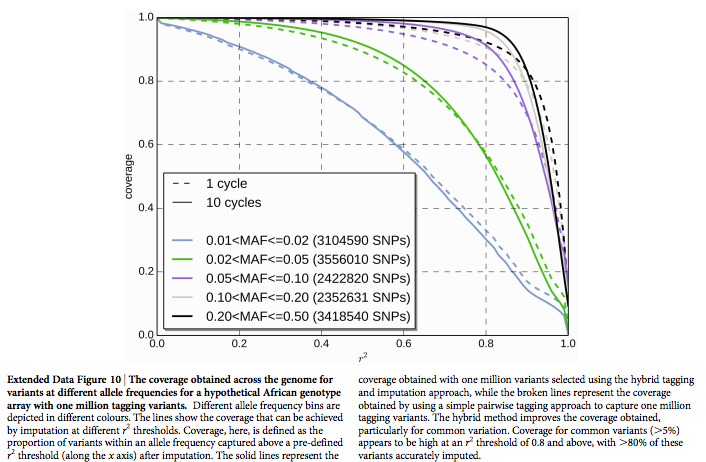
\includegraphics{fig/f10}
\caption[Imputation accuracy for a hypothetical 1M SNP array.]{
The coverage obtained across the genome for variants at different allele frequencies for a hypothetical African genotype array with one million tagging variants. Different allele frequency bins are depicted in different colours. The lines show the coverage that can be achieved by imputation at different \gls{r2} thresholds. Coverage, here, is defined as the proportion of variants within an allele frequency captured above a pre-defined \gls{r2} threshold (along the x axis) after imputation. The solid lines represent the coverage obtained with one million variants selected using the hybrid tagging and imputation approach, while the broken lines represent the coverage obtained by using a simple pairwise tagging approach to capture one million tagging variants. The hybrid method improves the coverage obtained, particularly for common variation. Coverage for common variants (\gls{MAF} greater than 0.05) appears to be high at an \gls{r2} threshold of 0.8 and above, with 80\% of these variants accurately imputed.
}
\label{fig:f10}
\end{figure}